\section{Atoms}
 
 The focus regarding atoms has been on simulating heavy atoms using a simple ansatz for the trial wave function, and thus test its limits. Due to the important nature of atoms in nature, precise calculations which are believed to be very close to the exact result for the given Hamiltonian are done. These results will be featured as experimental results in the discussions. For heavier atoms, relativistic effects become important due to the high energies of the valance electrons. Hence atoms heavier than krypton have not been studied. The specifics regarding the model used for atoms are covered in Section \ref{sec:modelAtoms}.
 
\subsection{Ground State Energies}
 
 Table \ref{tab:AtomsRes} presents the ground state energy results for different atoms together with the experimental results. As expected, helium has the best match with the corresponding experimental result out of all the atoms. The relative precision of the heavier atoms are in the range $10^{-3}$ - $10^{-4}$, indicating that DMC performs equally well in all cases. However, the error in the calculations increases as the atoms become heavier. The calculations were done on a single node; running the calculations on several nodes with an increased number of walkers could reduce the error somewhat. 
 
 In comparison to quantum dots, where the VMC and DMC results were relatively similar, it is evident that VMC performs rather poorly compared to DMC for atoms. Unlike quantum dots, the atomic systems allow for unbound states. This implies that the atomic systems in this thesis have an additional approximation in the trial wave function due to the fact that all the orbitals represent bound states. Nevertheless, this only further demonstrate the strengths of DMC to predict accurate results without much knowledge of the system at hand.
 
\begin{table}
\begin{center}
\begin{tabular}{lp{2cm}cclc}
Atom & & $E_\mathrm{VMC}$ & \qquad $E_\mathrm{DMC}$ & \qquad\,\, Expt. & \qquad $\epsilon_\mathrm{rel}$\\
\hline\hline
\ \\
He & \qquad & -2.8903(2) & \qquad -2.9036(2) & \qquad $-2.9037$ & \qquad $3.44\cdot 10^{-5}$\\
\ \\
Be & \qquad & -14.145(2) & \qquad -14.657(2)  & \qquad $-14.6674$ & \qquad $7.10\cdot 10^{-4}$ \\
\ \\
Ne & \qquad & -127.853(2) & \qquad -128.765(4) & \qquad $-128.9383$ & \qquad $1.34\cdot 10^{-3}$  \\
\ \\
Mg & \qquad & -197.269(3) & \qquad -199.904(8) & \qquad $-200.054$ & \qquad $7.50\cdot 10^{-4}$  \\
\ \\
Ar & \qquad & -524.16(7) & \qquad -527.30(4) & \qquad $-527.544$ & \qquad $4.63\cdot 10^{-4}$  \\
\ \\
Kr & \qquad & -2700(5) & \qquad -2749.9(2) & \qquad $-2752.054976$ & \qquad $7.83\cdot 10^{-4}$  \\
\ \\
\end{tabular}
\caption{Ground state energies for Atoms calculated using Variational - and Diffusion Monte-Carlo. Experimental energies are listed in the last column. As we see, DMC is rather close to the experimental energy. The relative error $\epsilon_\mathrm{rel} = |E_\mathrm{DMC} - \mathrm{Expt.}|/|\mathrm{Expt.}|$ is as expected lowest in the case of helium. The experimental energies, that is, the best possible results available, are taken from Ref. \cite{AtomsExact} for He through Ar, and \cite{KryptonExact} for Kr. }
\label{tab:AtomsRes}
\end{center}
\end{table}
 
 
 \subsection{One-body densities}
 
 The one-body densities for the \textit{noble gases}, that is, the closed shell atoms, are presented in Figure \ref{fig:OBD_noble_Atoms_2D_combo}. Comparing these to the one-body densities for the alkaline earth metals, i.e.~$\mathrm{Be}$, $\mathrm{Mg}$, etc., in Figure \ref{fig:OBD_alkaline_Atoms_2D_combo}, it is clear that the noble gases have a more confined electron distribution. This corresponds well to the fact that noble gases do not form compound materials, i.e.~molecules \cite{UniversityPhysics}. The alkaline earth metals, on the other hand, are found naturally as parts of compound materials. The one-body densities of the alkaline earth metals spreading out in space are thus in excellent agreement with what is expected.
 
It is apparent that the VMC distribution and the pure distribution differ more in the case of alkaline earth metals than for noble gases. This implies that the trial wave function is better in the case of noble gases. To explain this phenomenon, it is important to realize that for closed shell systems, the energy needed to excite an electron into the next $n$-shell is higher than the energy needed to excite an electron to the next $l$-level in an open shell system. The result of this is that the contributions from the exited states to the total wave function in Eq.~(\ref{eq:MultiDeterminantTWF}) are higher for the alkaline earth metals than for the noble gases. The approximation made in this thesis is that the trial wave function consists of a single determinant, thus neglecting the contribution from excited states. This approximation is in other words better in the case of noble gases than for the alkaline earth metals.
 
 
 
 \begin{figure}
 \begin{center}
   \subfigure{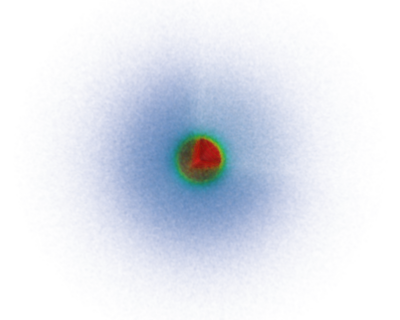
\includegraphics[scale=0.4]{../Graphics/OBD/OBD_Atoms/3D/Beryllium.png}} 
   \subfigure{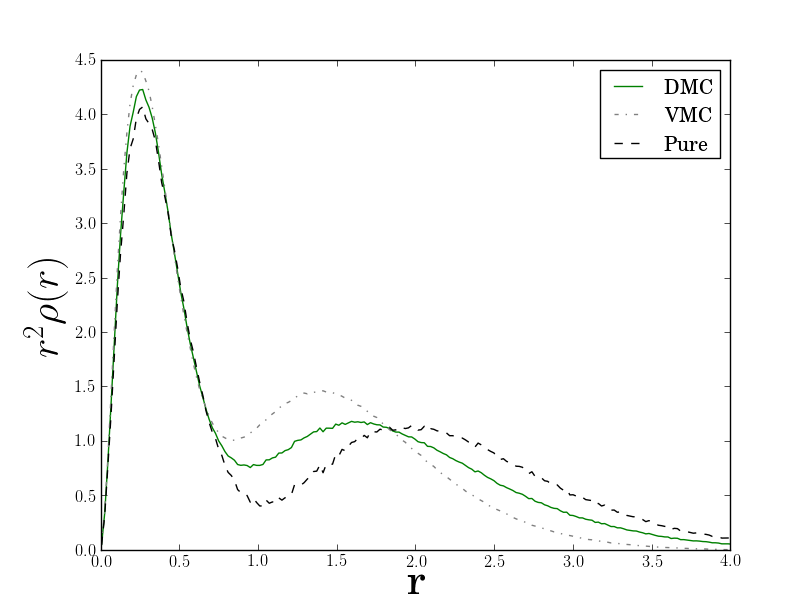
\includegraphics[scale=0.3]{../Graphics/OBD/OBD_Atoms/2D/Beryllium.png}}  \\
   \subfigure{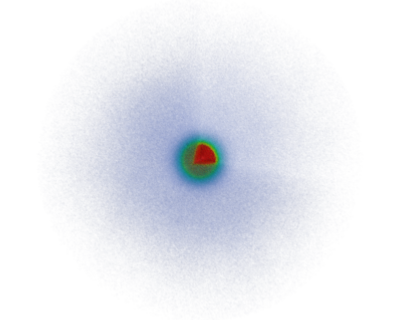
\includegraphics[scale=0.4]{../Graphics/OBD/OBD_Atoms/3D/Magnesium.png}} 
   \subfigure{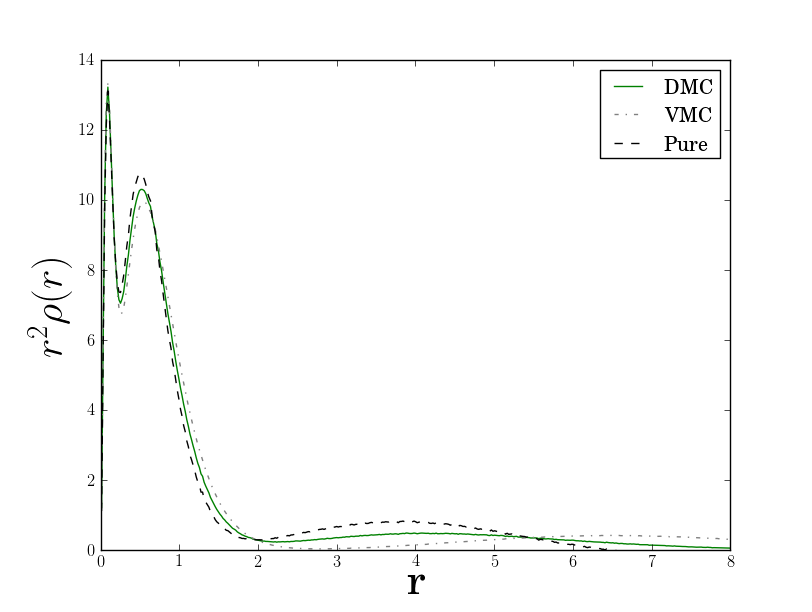
\includegraphics[scale=0.3]{../Graphics/OBD/OBD_Atoms/2D/Magnesium.png}}  \\
  \caption{Three dimensional one-body density (left column) and angular averaged radii (right column) for alkaline earth metals; beryllium (top) and magnesium (bottom). The color bar shows increasing values from left to right. Notice that the radial one-body density in the right column are multiplied by the radius squared. This is order to reveal the characteristics behind a density which otherwise is a generic peak around the origin. Compared to the noble gases in Figure \ref{fig:OBD_noble_Atoms_2D_combo}, the alkaline earth metals have a surrounding dispersed probability cloud due to the broken closed shell symmetry. The element is thus more unstable and potent for chemical reactions and molecular formations through covalent - and ionic bonds \cite{UniversityPhysics}. Red and blue color indicate a low and high electron density, respectively.}
  \label{fig:OBD_alkaline_Atoms_2D_combo}
 \end{center}
\end{figure}
 
\begin{figure}
 \begin{center}
   \subfigure{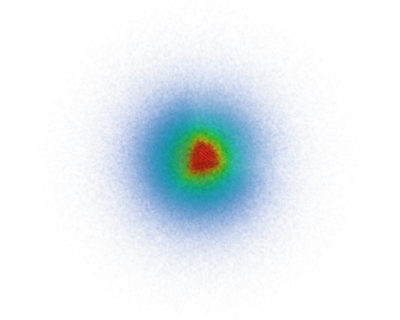
\includegraphics[scale=0.4]{../Graphics/OBD/OBD_Atoms/3D/Helium.png}} 
   \subfigure{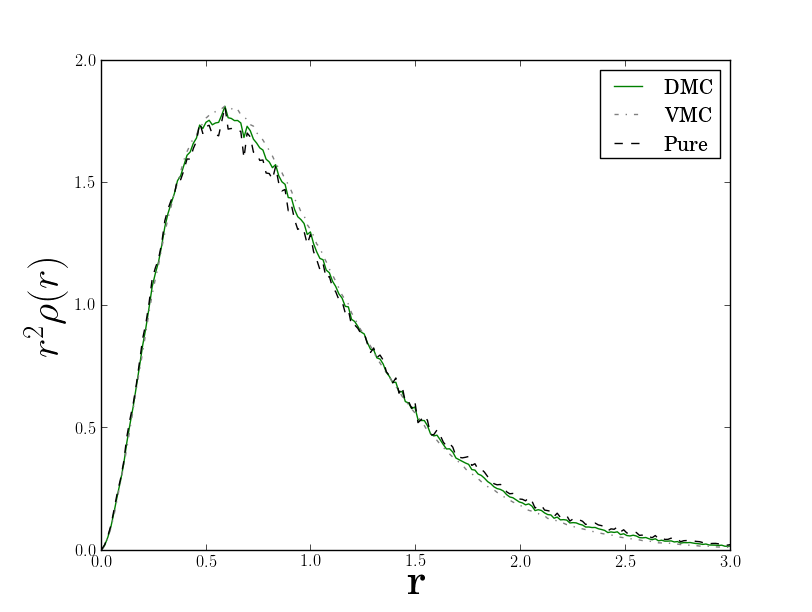
\includegraphics[scale=0.3]{../Graphics/OBD/OBD_Atoms/2D/Helium.png}}  \\
   \subfigure{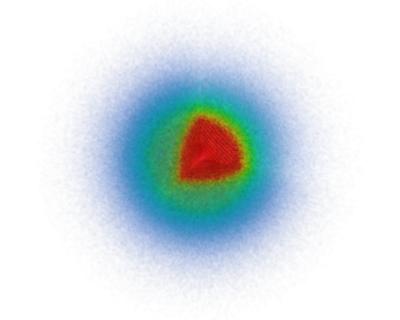
\includegraphics[scale=0.4]{../Graphics/OBD/OBD_Atoms/3D/Neon.png}} 
   \subfigure{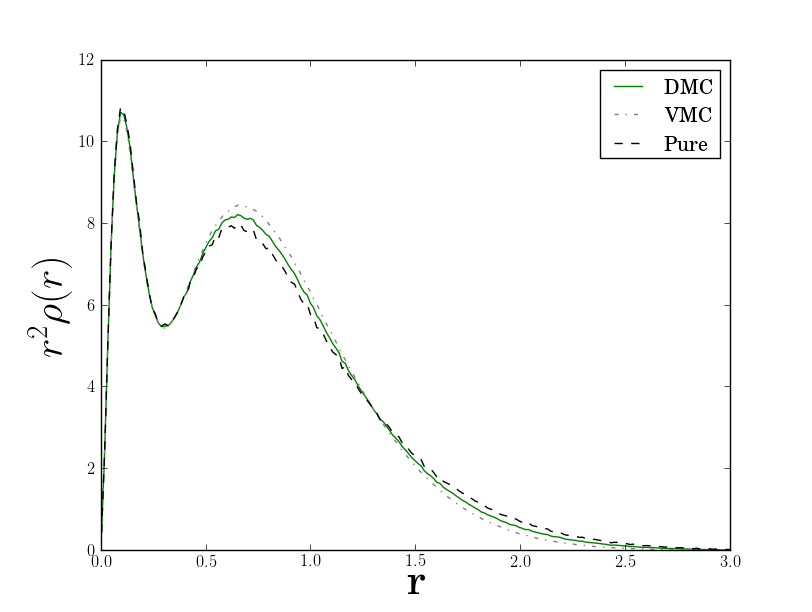
\includegraphics[scale=0.3]{../Graphics/OBD/OBD_Atoms/2D/Neon.png}}  \\
   \subfigure{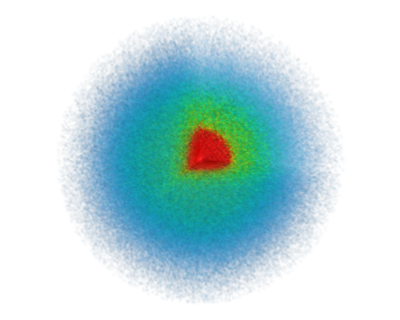
\includegraphics[scale=0.4]{../Graphics/OBD/OBD_Atoms/3D/Argon.png}} 
   \subfigure{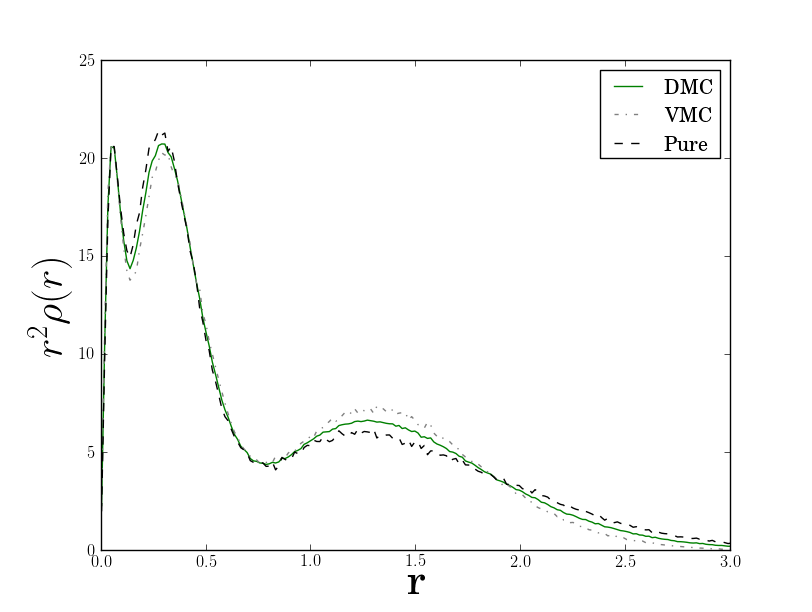
\includegraphics[scale=0.3]{../Graphics/OBD/OBD_Atoms/2D/Argon.png}}  \\
   \subfigure{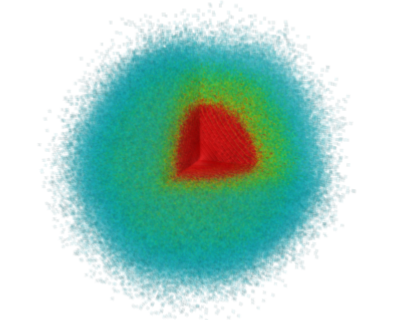
\includegraphics[scale=0.4]{../Graphics/OBD/OBD_Atoms/3D/Krypton.png}} 
   \subfigure{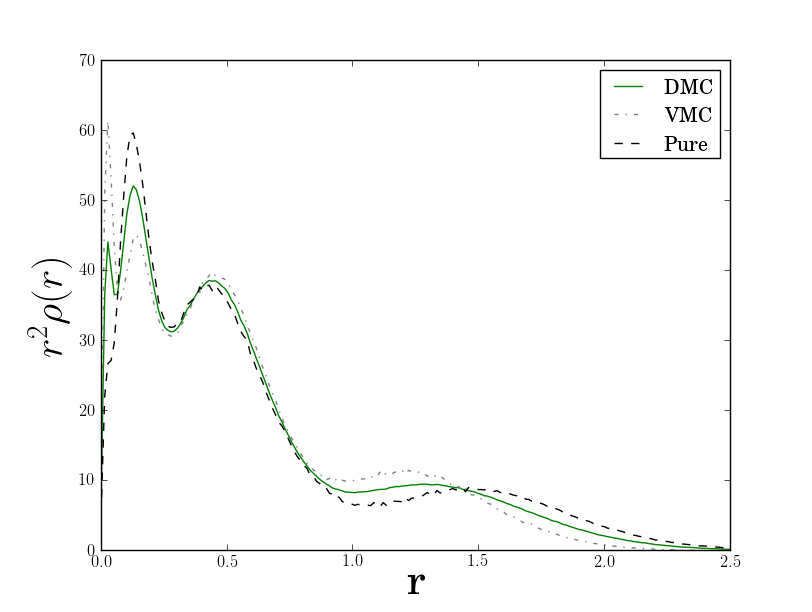
\includegraphics[scale=0.3]{../Graphics/OBD/OBD_Atoms/2D/Krypton.png}}  \\
  \caption{One-body densities for noble gases. Counting top to bottom: Helium, neon, argon and krypton. A quarter of the spherical density is removed to present a better view of the core. Red and blue color indicate a low and high electron density, respectively. Note that the radial densities are scaled with $r^2$ in order to reveal their differences. Unlike previous figures, the left and right column should thus not agree.}
  \label{fig:OBD_noble_Atoms_2D_combo}
 \end{center}
\end{figure}
 
 
